\section{Spannungsfolger mit LM358}
\subsection{Aufgabenstellung}
Die Schaltung aus Abbildung \ref{fig:Spannungsfolger_LM358_Schaltung} ist auf einem Steckbrett aufzubauen. Danach ist der Verstärker in die negative Versorgungsspannnung zu übersteuern. Dieses Verhalten ist aufzuzeichnen. 
\begin{figure}[H]
    \centering
    \begin{circuitikz}[]
        \draw (0,0) node[op amp] (opamp) {$LM358$};
        \draw (opamp.up) --++(0,0.5) node[vcc]{$V_{CC}$};
        \draw (opamp.down) --++(0,-0.5) node[vee]{$V_{EE}$};
        \draw (opamp.+) to[short,-o] ++(-2,0) node[left] {$U_{In}$};
        \draw (opamp.out) to[short,-o] ++(2,0) node[right] {$U_{a}$};
        \draw (opamp.-) to[short] ++(-1,0)
            to[short] ++(0,2)
            to[short] ++(4,0)
            to[short,-*] ++(0,-2.5);
        \end{circuitikz}
    \caption{Spannungsfolger mit LM358}
    \label{fig:Spannungsfolger_LM358_Schaltung}
 \end{figure}

\subsection{Messaufbau}
Zur Messung der oben genannten Schaltung wurde die Schaltung mit $V_{CC} = 10V$ und $V_{EE} = -7V$ versorgt. Da das Verhalten bei Übersteuerung gezeigt werden sollte und der verwendete Signalgenerator eine maximale $V_{PP} = 20V$ bereitstellen kann, musste hier eine geringere Versorgungspannung als bei vorherigen Messaufbauten verwendet werden
\begin{figure}[H]
    \centering
    \begin{circuitikz}[]
        \draw (0,0) node[op amp] (opamp) {$LM358$};
        \draw (opamp.up) --++(0,0.5) node[vcc]{$V_{CC}$};
        \draw (opamp.down) --++(0,-0.5) node[vee]{$V_{EE}$};
        \draw (opamp.+) to[short,-o] ++(-1,0) 
            %%Einfügen der Messschaltung
            to[sV=CH1, color=white, name=S1,o-o] ++(0,-2) node[ground] {}
            to[short,o-] ++(-2,0)
            to[sV] ++(0,2)
            to[short,-o] ++(2,0);
        \draw (opamp.out) to[short,-o] ++(2,0)
            %Einfügen der Messchaltung
            to[sV=CH2, color=white, name=S2,o-o] ++(0,-2) node[ground]{};
        \draw (opamp.-) to[short] ++(-1,0)
            to[short] ++(0,2)
            to[short] ++(4,0)
            to[short,-*] ++(0,-2.5);
        \myscope{S1}{0}
        \myscope{S2}{0}
        \end{circuitikz}
    \caption{Spannungsfolger mit LM358, Messaufbau zur Bestimmung des zeitlichen Verhaltens}
    \label{fig:Spannungsfolger_LM358_Messaufbau_Offset}
 \end{figure}

\subsection{Interpretation der Messergebnisse}
Der LM358 zeigt bei Aussteurung über den negatigen Gleichtaktaussteuerbereich eine sogenannte Phasenumkehr. Bei der Messung welche in Abbildung \ref{fig:LM358_Phasenumkehr} dargestellt ist, ist gut zu sehen, dass bei Aussteuerung über der Übersteuerung das Signal nicht einfach geklippt wird, sondern eine Phasenumkehr stattfindet. Das heißt konkret, dass in diesem Fall die positive, statt der negativen Versorgungspannung anliegt. 
\begin{figure}[H]
    \centering
    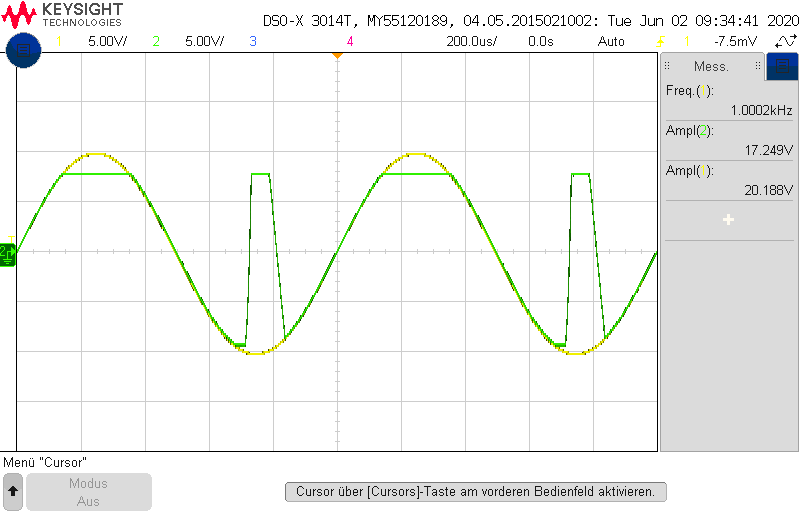
\includegraphics[width=\textwidth]{Lab_2/Messungen/Follower/scope_35.png}
    \caption{LM358 Phasenumkehr bei negativer Übersteuerung}
    \label{fig:LM358_Phasenumkehr}
\end{figure}

%%%%%%%%%%%%%%%%%%%%%%%%%%%%%%%%%%%%%%%%%%%%%%%%%%%%%%%%%%%%%%%%%%%%%%%%%%%%%%%%%%%%%%%%%%%%%%%%%%%%%%%%%%%%%%%%%%%%%%%%%%%%%%
\section{Tiefpass erster Ordnung mit LM358}
\subsection{Aufgabenstellung}
Die in Abbildung \ref{fig:aktiver_Tiefpass_LM358_Schaltung} dargestellte Tiefpassschaltung ist auf eine $f_g=1kHz$ und eine Verstärkung im Durchlassbereich von $\nu = -10$ auszulegen. Die Schaltung ist auf dem Steckbrett aufzubauen.

Danach sind die Grenzfrequenz und die Verstärkung, das Verhalten bei nicht-sinusförmigen Eingangsspannungen und ein Bodediagramm messtechnisch zu erfassen. 
\begin{figure}[H]
    \centering
    \begin{circuitikz}[]
        \draw (0,0) node[op amp] (opamp) {$LM358$};
        \draw (opamp.up) --++(0,0.5) node[vcc]{$V_{CC}$};
        \draw (opamp.down) --++(0,-0.5) node[vee]{$V_{EE}$};
        \draw (opamp.+) to[short] ++(-0.5, 0) to[short] ++(0, -0.5) node[ground]{}; 
        
        \draw (opamp.-) to[R=$R_1$,-o] ++(-2,0) node[left]{$U_{in}$};
        \draw (opamp.-) to[short, *-] ++(0,2)
            to[R=$R_2$,*-*] ++(3,0)
            to[short,-*] ++(0,-2.5)
            to[short] (opamp.out);
        \draw (opamp.-) to[short, *-] ++(0,3.5)
            to[C=$C$] ++(3,0)
            to[short] ++(0,-2);
        \draw (opamp.out) to[short, -o] (3,0) node[right]{$U_{out}$};
        \end{circuitikz}
    \caption{aktiver Tiefpass erster Ordnung}
    \label{fig:Spannungsfolger_LM358_Schaltung}
 \end{figure}

\subsection{Messaufbau}
\begin{figure}[H]
    \centering
    \begin{circuitikz}[]
        \draw (0,0) node[op amp] (opamp) {$LM358$};
        \draw (opamp.up) --++(0,0.5) node[vcc]{$V_{CC}$};
        \draw (opamp.down) --++(0,-0.5) node[vee]{$V_{EE}$};
        \draw (opamp.+) to[short] ++(-0.5, 0) to[short] ++(0, -0.5) node[ground]{}; 
        
        \draw (opamp.-) to[R=$R_1$] ++(-3,0)
            to[sV=CH1, color=white, name=S1,o-o] ++(0,-2) node[ground] {}
            to[short,o-] ++(-2,0)
            to[sV] ++(0,2)
            to[short,-o] ++(2,0);
        \draw (opamp.-) to[short, *-] ++(0,2)
            to[R=$R_2$,*-*] ++(3,0)
            to[short,-*] ++(0,-2.5)
            to[short] (opamp.out);
        \draw (opamp.-) to[short, *-] ++(0,3.5)
            to[C=$C$] ++(3,0)
            to[short] ++(0,-2);
        \draw (opamp.out) to[short, -o] (3,0) 
            to[sV=CH2, color=white, name=S2,o-o] ++(0,-2) node[ground]{};
        
        \myscope{S1}{0}
        \myscope{S2}{0}
        \end{circuitikz}
    \caption{Messaufbau, aktiver Tiefpass erster Ordnung}
    \label{fig:Spannungsfolger_LM358_Schaltung}
 \end{figure}

\subsection{Auslegung der Schaltung}
Bei der Auslegung der Schaltung wurde mit der Berechnung des Widerstandverhältnisses für die Verstärkung begonnen. Danach konnte die Grenzfrequenz der Schaltung mit der Kapazität $C$ bestimmt werden.

\begin{align}
    \nu = -\frac{R_2}{R_1} &= -10\\
    R_1 = 1k\Omega \Rightarrow R_2 &= 10k\Omega\\
    C = \frac{1}{2\pi f_g R_1} &= 15,9nF
\end{align}

\subsection{Interpretation der Messergebnisse}
\begin{figure}[H]
    \centering
    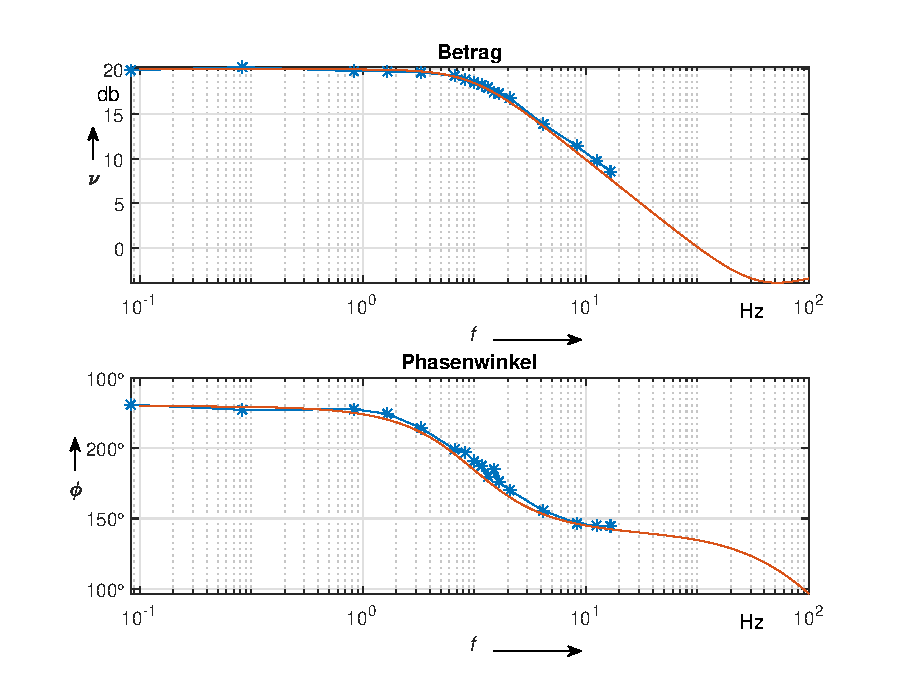
\includegraphics[width=\textwidth]{Lab_2/Plots/TP_first_order.eps}
    \caption{Bodediagramm des Tiefpasses erster Ordnung}
    \label{fig:Bode_aktiver_Tiefpass}
\end{figure}
In diesem Plot ist zu erkennen, dass die Grenzfrequenz bei der Simulation als auch bei den gemessenen Werten bei $f_g = 1kHz$ liegt. 

Der nächste Schritt war der Betrieb der Schaltung mit nicht-sinusförmigen Eingangsspanungen. Konkret wurde hier eine Rechteck und eine Dreieckspannung verwendet.

Um zu verstehen welche Messergebnisse hier zu erwarten sind, sollte an dieser Stelle ein Blick in die Übertragungsfunktion dieser Schaltung gewagt werden.

\begin{align}
    A = -\frac{R_2}{R_1}\frac{1}{1+sR_2 C}
\end{align}
Hier ist an dem Term $\frac{1}{s} $ zu erkennen, dass diese Schaltung integrierendes Verhalten zeigen muss. Durch Kenntnis der unbestimmten Integrale der Eingangsspannungen lassen sich nun Aussagen über die zu erwartenden Ausgangsspannungen treffen.
\subsubsection{Rechteckspannung}
\begin{align}
    \int{1 du} = u + c
\end{align}
Das heißt dass in diesem Fall eine linear ansteigend und abfallende Ausgangsspannung anliegen sollte.

Bei Rechteckspannung die sehr viel kleiner sind als die Grenzfrequenz ist eine Kondensatorladekurve zu sehen, was ebenfalls zu erwarten ist. 

\begin{figure}[H]
    \centering
    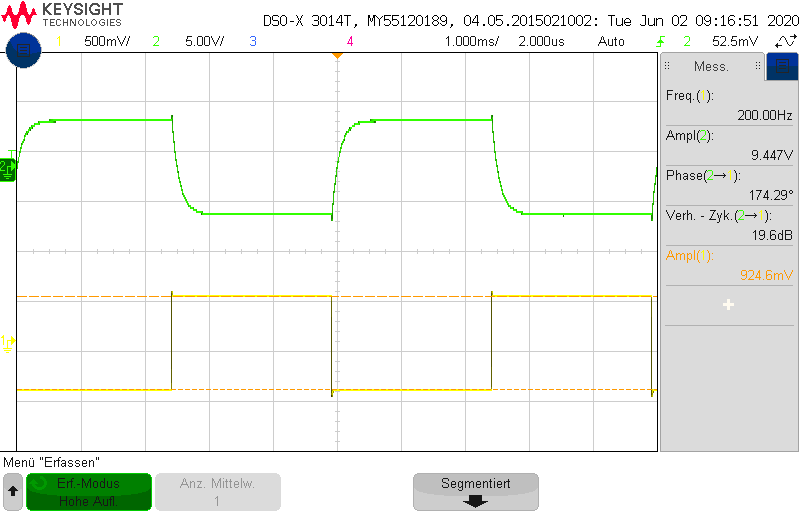
\includegraphics[width=\textwidth]{Lab_2/Messungen/TP_first_order/scope_26.png}
    \caption{Rechteckspannung beim Tiefpass erster Ordnung $f < f_g$}
    \label{fig:Rechteck_Tiefpass_erster_Ordnung_small_f}
\end{figure}
\begin{figure}[H]
    \centering
    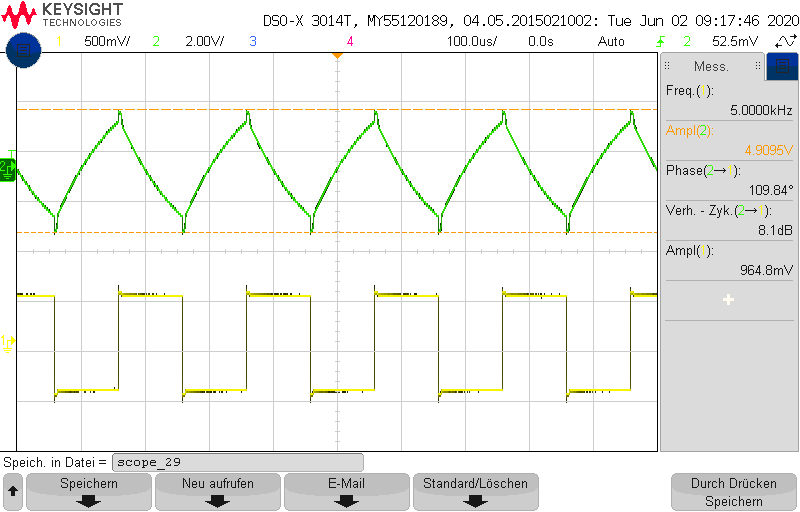
\includegraphics[width=\textwidth]{Lab_2/Messungen/TP_first_order/scope_29.png}
    \caption{Rechteckspannung beim Tiefpass erster Ordnung $f > f_g$}
    \label{fig:Rechteck_Tiefpass_erster_Ordnung_big_f}
\end{figure}

\subsubsection{Dreieckspannung}
Auch in diesem Fall kann die Übertragungsfunktion zu Rate gezogen werden um eine Aussage über die erwartete Ausgangsspannung zu treffen. Bei dieser Eingangsspannung ist lediglich eine anderes unbestimmtes Integral zu lösen.

\begin{align}
    \int{u du} = u^2 + c
\end{align}
Das heißt das nun eine Parabelförmige Ausgangsspannung am Ausgang zu erwarten ist.

\begin{figure}[H]
    \centering
    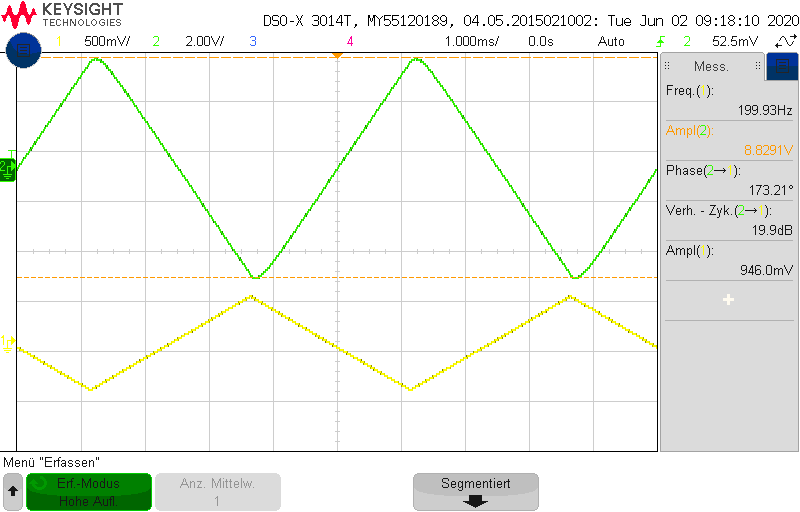
\includegraphics[width=\textwidth]{Lab_2/Messungen/TP_first_order/scope_30.png}
    \caption{Dreieckspannung beim Tiefpass erster Ordnung $f < f_g$}
    \label{fig:Dreieck_Tiefpass_erster_Ordnung_small_f}
\end{figure}
\begin{figure}[H]
    \centering
    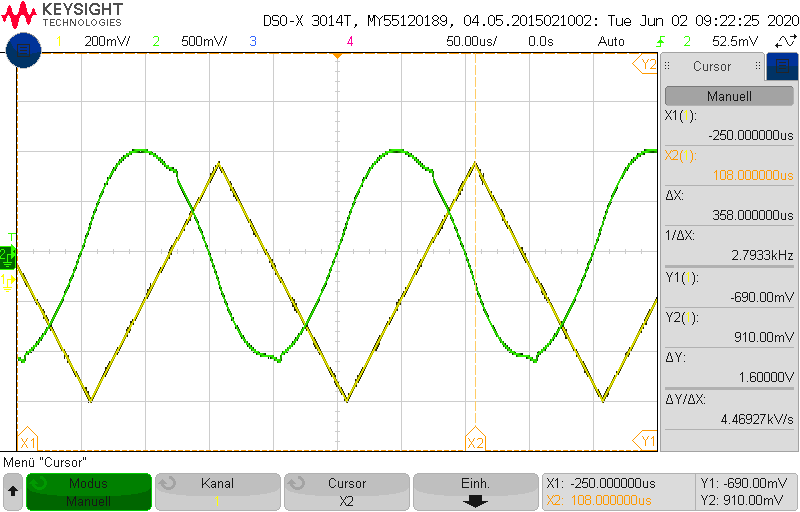
\includegraphics[width=\textwidth]{Lab_2/Messungen/TP_first_order/scope_34.png}
    \caption{Dreieckspannung beim Tiefpass erster Ordnung $f > f_g$}
    \label{fig:Dreieck_Tiefpass_erster_Ordnung_big_f}
\end{figure}
Wie zu erwarten ergab 8
\subsection{Ausarbeitungen}

%%%%%%%%%%%%%%%%%%%%%%%%%%%%%%%%%%%%%%%%%%%%%%%%%%%%%%%%%%%%%%%%%%%%%%%%%%%%%%%%%%%%%%%%%%%%%%%%%%%%%%%%%%%%%%%%%%%%%%%%%%%%%%
\section{Hochpass erster Ordnung mit LM358}
\subsection{Aufgabenstellung}
\begin{figure}[H]
    \centering
    \begin{circuitikz}[]
        \draw (0,0) node[op amp] (opamp) {$LM358$};
        \draw (opamp.up) --++(0,0.5) node[vcc]{$V_{CC}$};
        \draw (opamp.down) --++(0,-0.5) node[vee]{$V_{EE}$};
        \draw (opamp.+) to[short] ++(-0.5, 0) to[short] ++(0, -0.5) node[ground]{}; 
        
        \draw (opamp.-) to[R=$R_1$] ++(-2,0) to[C=$C$,-o]++(-2,0) node[left]{$U_{in}$};
        \draw (opamp.-) to[short, *-] ++(0,2)
            to[R=$R_2$] ++(3,0)
            to[short,-*] ++(0,-2.5)
            to[short] (opamp.out);

        \draw (opamp.out) to[short, -o] (3,0) node[right]{$U_{out}$};
        \end{circuitikz}
    \caption{aktiver Hochpass erster Ordnung}
    \label{fig:Hochpass_LM358_Schaltung}
 \end{figure}

\subsection{Messaufbau}
\begin{figure}[H]
    \centering
    \begin{circuitikz}[]
        \draw (0,0) node[op amp] (opamp) {$LM358$};
        \draw (opamp.up) --++(0,0.5) node[vcc]{$V_{CC}$};
        \draw (opamp.down) --++(0,-0.5) node[vee]{$V_{EE}$};
        \draw (opamp.+) to[short] ++(-0.5, 0) to[short] ++(0, -0.5) node[ground]{}; 
        
        \draw (opamp.-) to[R=$R_1$] ++(-2,0) to[C=$C$]++(-2,0) to[short] ++(-1,0)
            to[sV=CH1, color=white, name=S1,o-o] ++(0,-2) node[ground] {}
            to[short,o-] ++(-2,0)
            to[sV] ++(0,2)
            to[short,-o] ++(2,0);
            
        \draw (opamp.-) to[short, *-] ++(0,2)
            to[R=$R_2$] ++(3,0)
            to[short,-*] ++(0,-2.5)
            to[short] (opamp.out);

        \draw (opamp.out) to[short, -o] (3,0) to[sV=CH2, color=white, name=S2,o-o] ++(0,-2) node[ground]{};
        
        \myscope{S1}{0}
        \myscope{S2}{0}
        \end{circuitikz}
    \caption{aktiver Hochpass erster Ordnung}
    \label{fig:Hochpass_LM358_Messaufbau}
 \end{figure}

\subsection{Auslegung der Schaltung}

\subsection{Interpretation der Messergebnisse}

\subsection{Ausarbeitungen}